\documentclass{article}
\usepackage[utf8]{inputenc}
\usepackage{fullpage,amsmath,hyperref,indentfirst,graphicx,wrapfig,caption,subcaption,listings}
\graphicspath{{~/Desktop/JUPYTER-LAB}}
\lstset{columns = flexible, breaklines = true}
\date{}
\begin{document}
{\LARGE{\hskip 2.2 in CS170 Project 2}}
\vskip 0.5in
{\flushleft{Brandon Paulsen}}
{\flushleft{December 8$^\text{th}$, 2022}}
{\flushleft{UCR CS170 Fall 2022}}
{\flushleft{Professor Eamonn Keogh}}
\vskip 0.5in
\tableofcontents
\listoffigures
\pagebreak
\section{Introduction}
The goal of this project is to implement a feature selection algorithm in order to select (hopefully) optimal features for a nearest neighbor classifier on a large and small data set. Generally, nearest neighbor can be a very efficient classifier type, though it has a few shortcomings. Firstly, it can be very sensitive to errors in data labelling (a blue data point that was erroneously labelled as red, for example). Secondly, it is very sensitive to the features used. For example, if we consider a class "A" defined by those points that consists of pairs of integers such that the sum of the squares of the integers is greater than 10 and another class "B" that consists of pairs of integers such that the sum of the squares of the integers is less than 10, a nearest neighbor classifier considering any single integer of the elements of the classes (i.e. the first or the second integer) would be entirely useless, while considering both would yield fairly good results.
\par Theoretically, we could search the entire space of possible sets of features, but this would take much too long ($O(2^f)$ for $f$ being the number of features). In practice, we can use a combination of search with k-fold cross validation. There are two ways of doing this: starting with an empty set of features and building up greedily, and starting with a set of all possible features and greedily removing features one-by-one. For both of these methods, we will determine the optimal feature to add or remove by iterating over all options and comparing the result of k-fold cross validation. Both of these methods - that is the additive and subtractive methods - may seem fairly similar in their prospects, but as we will see later, one yields much more accurate results.
\section{Results}
\subsection{Small Data Results}
The small data for this project consisted of 500 instances with 6 features each (we are not told what sort of objects these are or what the features are). For the project, I was assigned small data set 61.
\subsubsection{Forward Selection}
Execution of the forward search feature selection algorithm on the small data set took 19.00 seconds. Maximal accuracy was found to be 0.976 using features 4 and 6. Progression of accuracy vs number of features can be seen in \textbf{Figure \ref{fig:Small Data Forward Selection Accuracy vs Features}}.
\begin{figure}[ht]
	\centering
	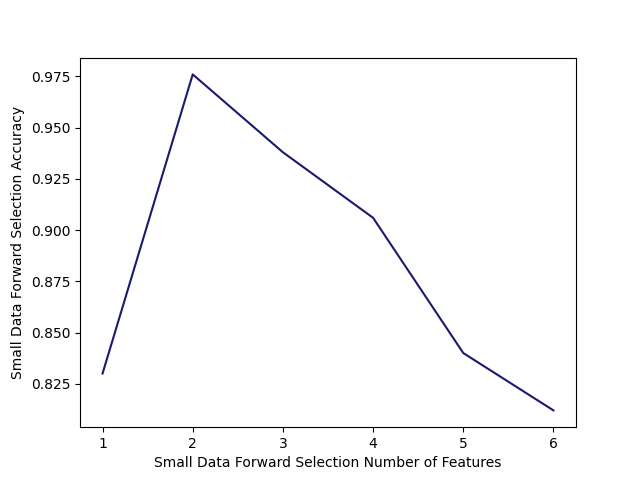
\includegraphics[width = 0.5\textwidth]{SmallDataForwardSelection.png}
	\caption{Small Data Forward Selection Accuracy vs Features}
	\label{fig:Small Data Forward Selection Accuracy vs Features}
\end{figure}
\subsubsection{Backward Selection}
Execution of the backward search feature selection algorithm on the small data set took 18.99 seconds. Maximal accuracy was found to be 0.976 using features 4,6 (same result as forward selection). Progression of accuracy vs number of features can be seen in \textbf{Figure \ref{fig:Small Data Backward Selection Accuracy vs Features}}.
\begin{figure}[ht]
	\centering
	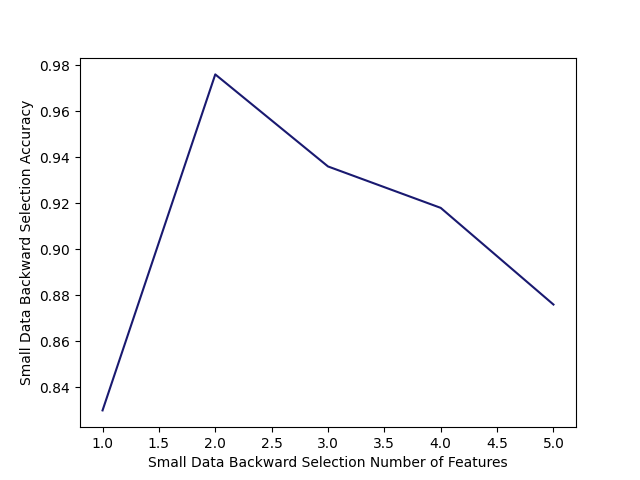
\includegraphics[width = 0.5\textwidth]{SmallDataBackwardSelection.png}
	\caption{Small Data Backward Selection Accuracy vs Features}
	\label{fig:Small Data Backward Selection Accuracy vs Features}
\end{figure}
\subsection{Large Data Results}
The large data for this project consisted of 1000 instances with 40 features each. I was assigned large dat set 33.
\subsubsection{Forward Selection}
Execution of the forward search feature selection algorithm on the large data set took 2988.38 seconds, or about 0.83 hours. Maximal accuracy was found to be 0.955 using features 22 and 34. Progression of accuracy vs number of features can be seen in \textbf{Figure \ref{fig:Large Data Forward Selection Accuracy vs Features}}.
\begin{figure}[ht]
	\centering
	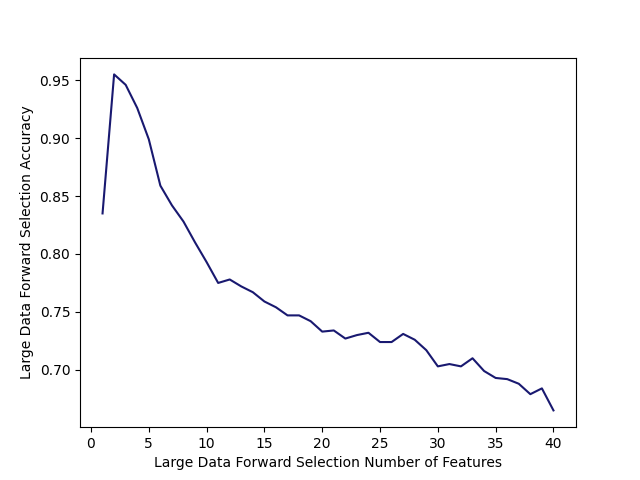
\includegraphics[width = 0.5\textwidth]{LargeDataForwardSelection.png}
	\caption{Large Data Forward Selection Accuracy vs Features}
	\label{fig:Large Data Forward Selection Accuracy vs Features}
\end{figure}
\subsubsection{Backward Selection}
Execution of the backward search feature selection algorithm on the large data set took 3167.73 seconds, or about 0.88 hours. Maximal accuracy was found to be 0.743 using features 4, 7, 12, 14, 15, 18, 20, 21, 23, 25, 26, 27, 28, 30, 32, 33, 35, 39, and 40. Progression of accuracy vs number of features can be seen in \textbf{Figure \ref{fig:Large Data Backward Selection Accuracy vs Features}}.
\begin{figure}[ht]
	\centering
	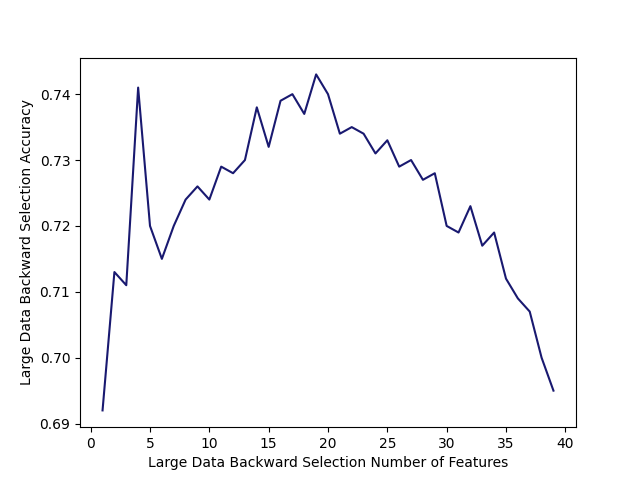
\includegraphics[width = 0.5\textwidth]{LargeDataBackwardSelection.png}
	\caption{Large Data Backward Selection Accuracy vs Features}
	\label{fig:Large Data Backward Selection Accuracy vs Features}
\end{figure}
\section{Conclusion}
For the small data, the forward selection and backward selection algorithms performed comparably, both in terms of accuracy and runtime. This is likely due to the fact that the total number of features and the number of relevant features are fairly similar (2 vs 6). Unfortunately, backward selection performed much worse on the large data than forward selection. This is likely due to there being many more irrelevant features, meaning large sets of features (those with many irrelevant features) are generally inaccurate and therefore, removing any singular feature from the set of all features makes little difference. Effectively, since we had so many irrelevant features, it was initially almost equally advantageous to remove any feature, and therefore the most effective features were removed before their benefit could be observed. This is supported by the plot of accuracy vs number of features being very noisy in \textbf{Figure \ref{fig:Large Data Backward Selection Accuracy vs Features}}.
\section{Code}
I wrote this project in python, then started to rewrite it in C++, assuming that python would be unimaginably slow. This was surprisingly not the case, as all trials took less than an hour to run, so I ended up scrapping my C++ version. The code for my project written in python can be found at \url{https://github.com/Poly1581/PYFeatureSelection}.
\pagebreak
\section{Program Output}
Trace output for the data sets assigned to me are included below. Some lines are much too wide for this document so they wrap around to the next line. I apologize for the ugliness that this induces.
\subsection{Small Data Output}
\lstinputlisting{SmallTrace.txt}
\pagebreak
\subsection{Large Data}
\lstinputlisting{LargeTrace.txt}
\end{document}
